ATLAS (A Toroidal L{\scshape hc} ApparatuS) is a general-purpose particle detector.
It contains several subdetector systems designed to measure different types of particles.
Starting from the beam line and working outwards, the Pixel Detector (PIX), Semiconductor Tracker (SCT), and Transition Radiation Tracker (TRT) make up the Inner Detector (ID) and are responsible for measuring the trajectories and momenta of charged particles.
Next are two calorimeters, the Liquid Argon Calorimeter (LAr) the Tile Calorimeter (TileCal), which stop electromagnetic and hadronic objects and measure their energies.
Finally, the outermost Muon Spectrometer (MS) measures muon tracks as they leave the detector, as they are too heavy to be stopped by the calorimeters.
The ATLAS detector and its subsystems are shown in Figure~\ref{fig:atlas}.

ATLAS uses a global, right-handed coordinate system with the origin at the center of the detector (the nominal interaction point).
The $x$-axis points from the origin inwards to the center of the LHC ring, the $y$-axis points upwards, and the $z$-axis points along the beam line.
Due to the azimuthal symmetry of the detector, it is useful to use cylindrical coordinates ($r,\phi$) in the plane transverse to the $z$-axis, where $\phi$ is the azimuthal angle.
Instead of using the polar angle $\theta$ to describe particle trajectories, pseudorapidity is used instead: %, defined in terms of $\theta$:
\begin{equation}
  \eta = -\mathrm{ln}\big(\mathrm{tan}(\theta/2)\big)\,.
  \label{eq:eta}
\end{equation}
Pseudorapidity has the useful property that differences in $\eta$ are invariant under Lorentz boosts along the $z$-axis.
The angular separation between two particles $p_i$ and $p_j$ is often expressed in terms of the quantity $\Delta R$, defined as
\begin{equation}
  \Delta R(p_i,p_j) = \sqrt{\Delta\eta_{i,j}^2 + \Delta\phi_{i,j}^2}\,,
  \label{eq:deltar}
\end{equation}
where $\Delta\phi_{i,j} \in [-\pi,\pi]$ since $\phi$ is periodic in $2\pi$ and ``wraps around'' the detector in the azimuthal direction.

\begin{figure}[tbp]
  \begin{center}
    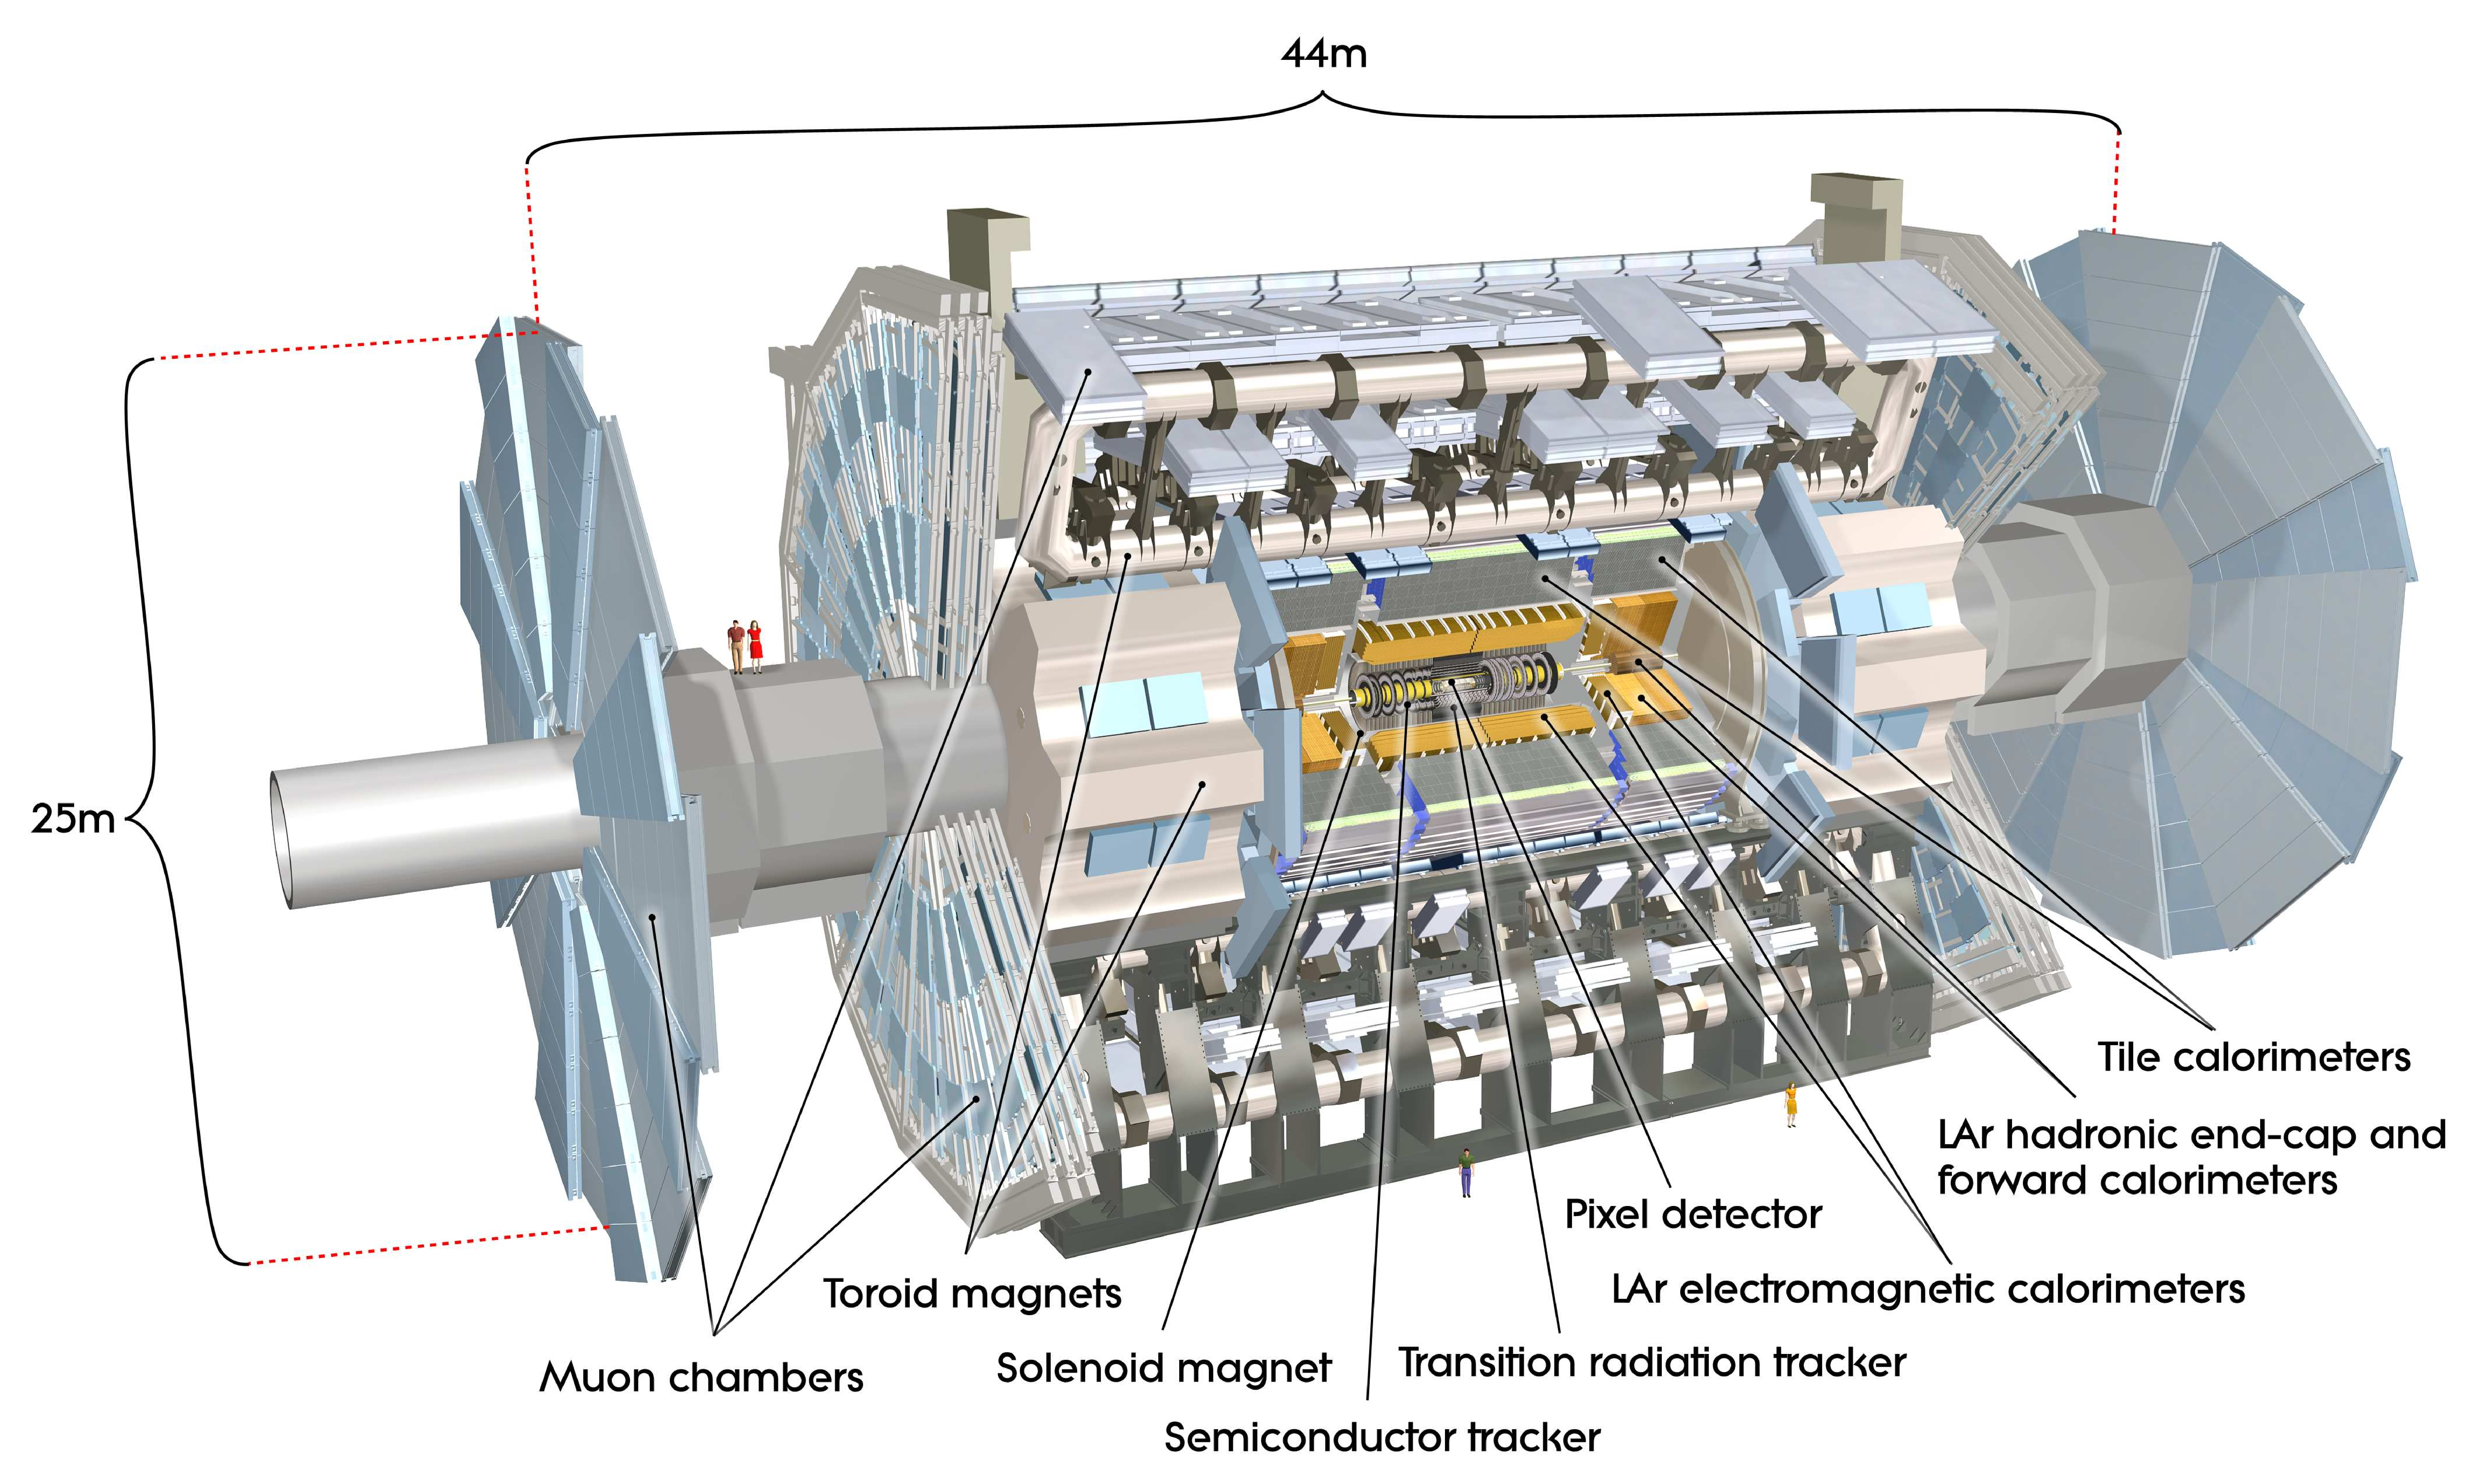
\includegraphics[width=0.98\textwidth]{figs/detector/atlas.pdf}
  \end{center}
  \caption[Cut-away view of the ATLAS detector.]{Cut-away view of the ATLAS detector~\cite{PERF-2007-01}.}
  \label{fig:atlas}
\end{figure}
